\documentclass[11pt,aspectratio=169]{beamer}
\usepackage[T1]{fontenc}
\usepackage{lmodern}
\usepackage{amsmath,amssymb,booktabs,graphicx}
\definecolor{Ink}{HTML}{23313D}
\definecolor{Accent}{HTML}{126B75}
\definecolor{Muted}{HTML}{67737C}
\definecolor{Warm}{HTML}{AD591D}
\setbeamercolor{normal text}{fg=Ink,bg=white}
\setbeamercolor{structure}{fg=Accent}
\setbeamercolor{frametitle}{fg=Ink}
\setbeamercolor{alerted text}{fg=Warm}
\setbeamerfont{frametitle}{size=\Large,series=\bfseries}
\setbeamerfont{title}{size=\LARGE,series=\bfseries}
\setbeamersize{text margin left=8mm,text margin right=8mm}
\setbeamertemplate{navigation symbols}{}
\setbeamertemplate{itemize item}{\small\raise1pt\hbox{\textcolor{Accent}{\textbullet}}}
\setbeamertemplate{frametitle}{\vspace{3mm}\insertframetitle\par\vspace{1mm}{\color{Accent}\hrule height .5pt}\vspace{2mm}}
\setbeamertemplate{footline}{\hspace{8mm}\textcolor{Muted}{\scriptsize Acemoglu, Kong \& Ozdaglar (2026)}\hfill\textcolor{Muted}{\scriptsize\insertframenumber\,/\,\inserttotalframenumber}\hspace{8mm}\vspace{3mm}}
\newcommand{\source}[1]{\par\vspace{2mm}{\scriptsize\color{Muted}#1}}
\newcommand{\claim}[1]{{\color{Accent}\bfseries #1}\par\medskip}
\newcommand{\photopanel}[1]{%
\IfFileExists{#1}{\includegraphics[width=\linewidth,height=4.05cm,keepaspectratio]{#1}}{%
\fbox{\begin{minipage}[c][3.8cm][c]{.88\linewidth}\centering
\textcolor{Warm}{\textbf{Handwritten photo pending}}\par\medskip
\small Derive $g'$, $U_{eX}$ and $U_{e\tau_A}$ on paper.\par\medskip
Photograph your work and save it as\par\texttt{hand/derivation.jpg}.\par\medskip
\scriptsize This panel is not evidence of handwritten work.
\end{minipage}}}}

\title{Better advice, weaker learning?}
\author{Acemoglu, Kong and Ozdaglar (2026)}
\begin{document}
\begin{frame}
\vspace{5mm}
{\color{Accent}\small EXTENDED READING AND STATIC VERIFICATION}\par\bigskip
{\usebeamerfont{title}\inserttitle}\par\medskip
{\large AI, Human Cognition and Knowledge Collapse}\par\bigskip
Acemoglu, Kong and Ozdaglar\par
NBER Working Paper 34910, February 2026\par\bigskip
\href{https://github.com/gsaco/ai-04-acemoglu}{\textcolor{Accent}{github.com/gsaco/ai-04-acemoglu}}
\source{Static derivations and an original assumption test.\newline
Dynamic and welfare results are reported from the paper, not reproduced.}
\end{frame}

\begin{frame}{The bridge: private decisions create public information}
\claim{The information that saves effort today can weaken learning tomorrow.}
\begin{itemize}\setlength\itemsep{4mm}
\item A person needs general understanding and context-specific information.
\item Human effort improves their own information and leaves a public trace.
\item Personalized AI replaces part of the private reason to learn.
\item That response can reduce the public knowledge inherited by later cohorts.
\end{itemize}
\source{Introduction; \S2, pp. 5--6: the contribution combines individual information acquisition\newline
with collective learning, rather than treating collaboration as a single isolated task.}
\end{frame}

\begin{frame}{Production: complementarity is an assumption}
Let $b_G,b_I\in\{0,1\}$ indicate prediction errors within a unit band.
\[
 f(b_G,b_I)=f(0,0)+\Delta_G b_G+\Delta_I b_I+\Delta_X b_Gb_I.
\]
\[
\begin{aligned}
\Delta_G&=f(1,0)-f(0,0),\\
\Delta_I&=f(0,1)-f(0,0),\\
\Delta_X&=f(1,1)-f(1,0)-f(0,1)+f(0,0).
\end{aligned}
\]
Monotone $f$; $\Delta_G+\Delta_I+\Delta_X=1$.
\medskip

\textbf{Assumption 1:} $\Delta_I=0$, $\Delta_X>0$.
General knowledge is essential for context-specific information to pay off.
\source{\S3.1, p. 8. Leontief is one example ($\Delta_G=\Delta_I=0$, $\Delta_X=1$), not the entire model.}
\end{frame}

\begin{frame}{Normal information: precisions add}
The common state drifts; the individual state is fresh each period:
\[
\theta_{t+1}=\theta_t+\varepsilon_t,\quad\varepsilon_t\sim N(0,\Sigma^2),
\qquad \theta_{i,t}\sim N(0,\sigma^2).
\]
Independent human and AI signals about the individual state give
\[
\boxed{Y=\sigma^{-2}+\lambda_I e+\tau_A.}
\]
\textbf{Public information:} $X=\operatorname{Var}(\theta_t\mid\mathcal I_t)^{-1}$.
It is inherited when effort is chosen.
\medskip

Posterior means maximize the probability of lying within the symmetric
unit-tolerance band. The two success probabilities are $G(X)$ and $G(Y)$.
\source{\S\S3.1--3.3, pp. 7--12, eqs. (4)--(5). Gaussian, conditionally independent information.}
\end{frame}

\begin{frame}{The static objective and its unique optimum}
Dropping $f(0,0)$, and using $\Delta_I=0$:
\[
U=G(X)\Delta_G+G(X)G(Y)\Delta_X-e^\alpha/\alpha.
\]
\[
\boxed{\Delta_XG(X)\lambda_I g(Y)=e^{\alpha-1}.}
\]
For $e>0$,
\[
U_{ee}=\Delta_XG(X)\lambda_I^2g'(Y)-(\alpha-1)e^{\alpha-2}<0.
\]
At $X>0$, marginal benefit at zero is positive, while marginal cost
ultimately dominates: a unique, finite, interior optimum exists.
\source{\S3.5, p. 14. Conditions: $\alpha>1$, $\lambda_I>0$, $\Delta_X>0$,\newline
$\sigma^{-2}>0$, finite $\tau_A\geq0$. At $X=0$, the optimum is the boundary $e=0$.}
\end{frame}

\begin{frame}{Deriving the two signs by hand}
\[
G(z)=2\Phi(\sqrt z)-1,\qquad g(z)=\frac{e^{-z/2}}{\sqrt{2\pi z}}.
\]
Log-differentiation makes the curvature transparent:
\[
\frac{g'(z)}{g(z)}=-\frac12-\frac{1}{2z}<0.
\]
\[
\begin{aligned}
 U_{eX}&=\Delta_X\lambda_I g(X)g(Y)>0,\\[2mm]
 U_{e\tau_A}&=\Delta_XG(X)\lambda_I g'(Y)<0.
\end{aligned}
\]
\textbf{Interpretation:} $X$ increases the value of private precision; $\tau_A$
reduces its marginal value by already supplying it.
\source{Observation 1, p. 13. Strict signs on $X,Y>0$ with $\Delta_X,\lambda_I>0$;\newline
short-lived atomistic agents do not internalize their public learning contribution.}
\end{frame}

\begin{frame}{From payoff cross-partials to effort responses}
Differentiate the interior FOC $U_e(e^*,X,\tau_A)=0$:
\[
 e_X^*=-\frac{U_{eX}}{U_{ee}}>0,
 \qquad e_{\tau_A}^*=-\frac{U_{e\tau_A}}{U_{ee}}<0.
\]
\claim{The denominator matters: substitution is a choice result because the optimum is concave.}
\begin{itemize}\setlength\itemsep{3mm}
\item These derivatives hold at fixed inherited $X$ or fixed $\tau_A$.
\item Aggregation capacity $I$ is absent from the current private FOC.
\item $I$ matters through the public information later cohorts inherit.
\end{itemize}
\source{Observation 2, p. 14; own implicit-function derivation.\newline
Do not confuse the technology parameter $\lambda_I$ with island size $I$.}
\end{frame}

\begin{frame}{The Bayesian bridge, read without solving dynamics}
The paper's public-information recursion is
\[
V_{t+1}=\frac{1}{X_t+\lambda_G I e_t}+\Sigma^2,
\qquad
X_{t+1}=\left[\frac{1}{X_t+\lambda_G I e_t}+\Sigma^2\right]^{-1}.
\]
\begin{itemize}\setlength\itemsep{4mm}
\item Pooling human signals adds \textbf{precision}: $\lambda_G I e_t$.
\item State innovation adds \textbf{variance}: $\Sigma^2$.
\item The static best response supplies $e_t=e(X_t,\tau_A)$.
\end{itemize}
\source{\S3.2, eq. (3), p. 11; Proposition 1, p. 15.\newline
Reported model equation only: no recursion simulation or steady-state reconstruction.}
\end{frame}

\begin{frame}{What the dynamic results claim}
\small
Assumption 1; $I,\lambda_I,\lambda_G,\Sigma^2,\sigma^2>0$; finite $\tau_A\geq0$.
\medskip

\begin{tabular}{@{}p{.26\textwidth}p{.68\textwidth}@{}}
\toprule
Cost regime & Reported result \\
\midrule
$\alpha-1>1/4$ & Zero is unstable; one positive stable steady state attracts every $X_1>0$. Zero remains a fixed point. \\[3mm]
$0<\alpha-1<1/4$ & Below $\tau_A^c$, zero and a high state are stable, separated by $\bar X_m$. Above $\tau_A^c$, only zero remains. \\
\bottomrule
\end{tabular}
\medskip

In the second regime, $X_1>\bar X_m$ selects the high state;
$X_1<\bar X_m$ selects collapse. At $X_1=\bar X_m$, the state stays there.
\medskip

\textbf{Boundary discipline:} these claims exclude $\alpha-1=1/4$.
We use strict inequalities around $\tau_A^c$; the paper's treatment of equality is inconsistent.
\source{Propositions 3 and 5, pp. 18, 20; see extra/analysis.md for the threshold caveat.}
\end{frame}

\begin{frame}{Welfare: which quantity is being differentiated?}
\textbf{Static optimized utility} $v(X,\tau_A)=\max_e U(e;X,\tau_A)$:
\[
\left.\frac{\partial v}{\partial\tau_A}\right|_X=G(X)\Delta_Xg(Y)>0.
\]
\textbf{High-steady-state welfare}, as reported in the paper:
\[
\frac{d\bar U^+}{d\tau_A}
=\underbrace{G(\bar X_h)\Delta_Xg(\bar Y_h)}_{\text{direct gain}}
+\underbrace{g(\bar X_h)[\Delta_G+G(\bar Y_h)\Delta_X]
\frac{d\bar X_h}{d\tau_A}}_{\text{loss of public knowledge}}.
\]
\claim{Private improvement at fixed knowledge does not imply a social long-run improvement.}
\source{Static envelope calculation: own verification. Long-run decomposition: \S4.3, p. 25.\newline
Welfare is output minus effort cost, relative to $f(0,0)$; dynamic results are read-only.}
\end{frame}

\begin{frame}{Welfare theorems: the qualifications are the result}
\small
\textbf{Common conditions:} baseline model and Assumption 2,
$\sigma^{-2}\geq\sqrt2-1$; other parameters held fixed.
\medskip

\textbf{Proposition 10:} if $\alpha-1>1/4$, a finite $\tau_A^*\geq0$ maximizes
$\bar U^+$. Welfare increases below it, decreases above it, and tends to zero
as $\tau_A\to\infty$. Realized high-state welfare requires $X_1>0$.
\medskip

\textbf{Proposition 11:} if $0<\alpha-1<1/4$ and the positive branch exists,
$0\leq\tau_A^*<\tau_A^c$. Welfare on that branch increases then decreases;
above $\tau_A^c$ the collapse outcome has zero normalized welfare.
Realized welfare also depends on the initial basin.
\medskip

\textbf{Not necessarily interior:} $\tau_A^*=0$ is explicitly allowed.
Without Assumption 2, the paper discusses failure of single-peakedness.
\source{\S4.1, pp. 23--24; Assumption 2 and footnote 6, p. 25; Propositions 10--11, p. 26.\newline
When no positive branch exists even at zero AI precision, do not assert a positive-branch optimum.}
\end{frame}

\begin{frame}{Section 5 changes information production}
\small
\begin{tabular}{@{}p{.22\textwidth}p{.70\textwidth}@{}}
\toprule
Extension & What changes and what is claimed \\
\midrule
5.1 Aggregation & $I(\tau_A)=I_0+e^{\eta\tau_A}$. For $\eta<1/[2(\alpha-1)]$, knowledge still tends to zero at very high AI precision. \\[3mm]
5.2 Synthetic data & Adds $0<\tau_{\rm syn}<\infty$ public precision each period. Least and greatest steady states are positive; effort and knowledge fall with $\tau_A$. \\[3mm]
5.3 Effort bundling & Public precision scales with $e^\beta$. For $\beta>0$, the stability comparison becomes $\alpha-1\gtrless\beta/4$. $\beta=0$ is exceptional. \\
\bottomrule
\end{tabular}
\medskip

\textbf{Never relaxed:} $\Delta_I=0$. Section 5.3 changes the public-learning
technology; it does not give context-specific knowledge standalone output value.
\source{\S5, Propositions 14--16, pp. 29--32. The formal \S5.3 extension has one effort choice,\newline
not a separately optimized allocation between two effort types.}
\end{frame}

\begin{frame}{My extension: give context-specific knowledge some value}
Allow $\Delta_I>0$, retain $\Delta_X>0$, and preserve normalization:
\[
U=\Delta_GG(X)+[\Delta_I+\Delta_XG(X)]G(Y)-e^\alpha/\alpha.
\]
\[
\begin{aligned}
 U_{eX}&=\Delta_X\lambda_I g(X)g(Y)>0,\\
 U_{e\tau_A}&=[\Delta_I+\Delta_XG(X)]\lambda_I g'(Y)<0.
\end{aligned}
\]
At the zero-knowledge boundary and finite $\tau_A$,
\[
\boxed{U_e(0;0,\tau_A)=\Delta_I\lambda_I g(\sigma^{-2}+\tau_A)>0.}
\]
\textbf{Verdict:} both signs survive; zero effort at zero knowledge does not.
This tests the essential-input assumption, without solving a new dynamic model.
\source{Own static extension, not a result stated by the authors.\newline
$\alpha>1$, $\lambda_I>0$, $\sigma^{-2}>0$, $\Delta_I>0$; choose $\Delta_G\geq0$ to keep monotonicity.}
\end{frame}

\begin{frame}{Reproducible evidence, not a calibration}
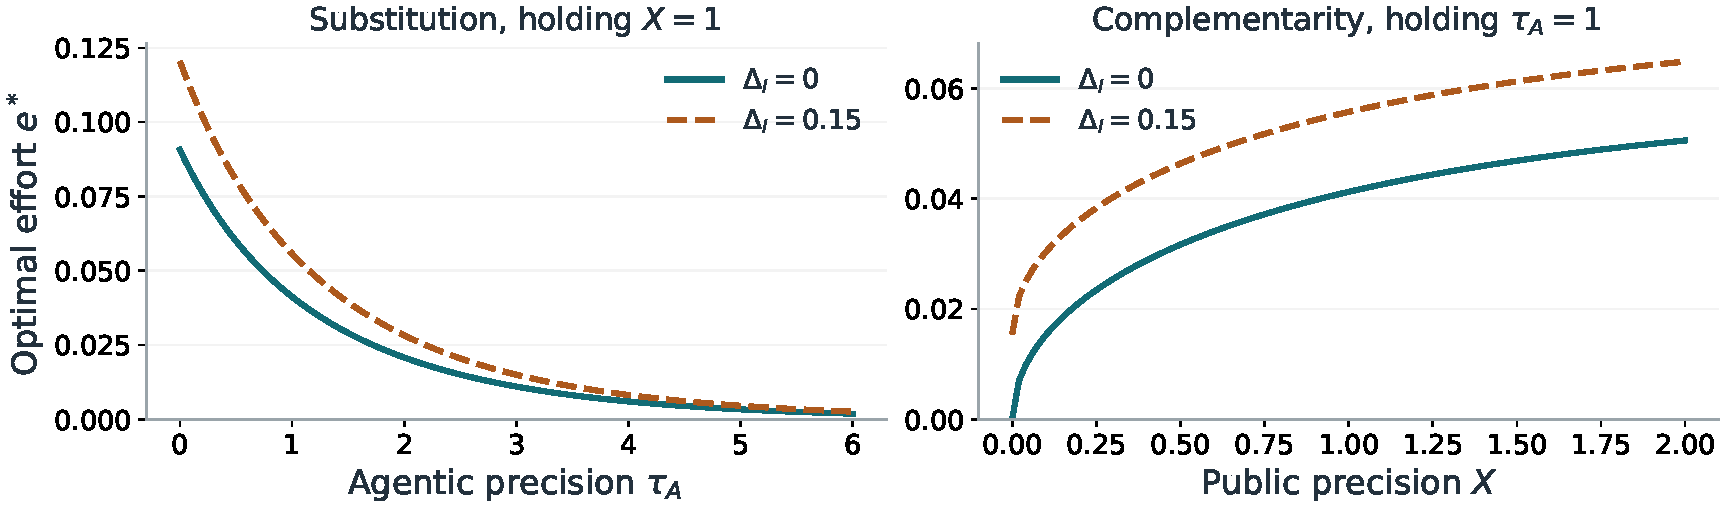
\includegraphics[width=\textwidth,height=3.5cm,keepaspectratio]{figures/static_checks.pdf}\par
\small
Six symbolic identities; 444 numerical optima; FOC residuals below
$2.5\times10^{-15}$. Implicit-function and envelope derivatives match finite differences.
\medskip

At $X=0$, $\tau_A=1$: $e^*=0$ under $\Delta_I=0$ versus $0.01539$ under $\Delta_I=.15$.
\source{extra/static\_checks.py; $\alpha=2$, $\lambda_I=\sigma^{-2}=1$, $\Delta_X=.6$, $\Delta_G=1-\Delta_I-\Delta_X$.\newline
Illustrative parameters only. No dynamic paths, collapse thresholds or welfare curves fitted.}
\end{frame}

\begin{frame}{Handwritten static derivation}
\begin{columns}[T]
\begin{column}{.45\textwidth}
\photopanel{../hand/derivation.jpg}
\end{column}
\begin{column}{.51\textwidth}
\small
\textbf{Derivation checklist:}\par\medskip
1. Differentiate $G$ and $g$.\par\medskip
2. Derive the FOC and both signs.\par\medskip
3. Add $\Delta_I G(Y)$ and evaluate the boundary marginal return.\par\medskip
\textbf{Own verdict to defend:}\par
The static crowd-out mechanism is robust to $\Delta_I>0$.
Exact zero-knowledge collapse and zero welfare rely on additional assumptions.
\end{column}
\end{columns}
\source{Student-provided photograph: hand/derivation.jpg. The photo documents the baseline derivatives and FOC; the extension and verdict remain to be documented by hand.}
\end{frame}

\begin{frame}{Limits, policy claims and questions for the oral}
\small
\textbf{Aggregation:} Proposition 9 raises high-state welfare with $I$, when that
state exists. Better aggregation and better agentic advice are different changes.
\medskip

\textbf{Policy, read-only:} Proposition 13 optimizes eventual Gaussian signal caps
under long-run average welfare, $0<\alpha-1<1/4$, Assumption 2,
and $X_1>\bar X_m(0)$. It is not an unrestricted or discounted policy theorem.
\medskip

\textbf{Questions to defend:}
\begin{itemize}
\item Why does zero effort follow at $X=0$? Because $\Delta_I=0$.
\item Does $\Delta_I>0$ reverse crowd-out? No, the negative cross-partial remains.
\item Does the example prove AI always improves long-run welfare? No.
\item Is an interior accuracy cap guaranteed? No; $\tau_A^*=0$ is allowed.
\end{itemize}
\source{Primary source throughout: supplied w34910.pdf, NBER WP 34910 (February 2026).\newline
Detailed conditions, derivations, evidence map and five-minute script: extra/analysis.md and extra/oral-notes.md.}
\end{frame}
\end{document}
